\documentclass{beamer}
\usepackage{mathrsfs,xcolor,setspace,comment,centernot,listings,framed,subfig,ragged2e}
\usepackage[utf8]{inputenc}
\usepackage[T1]{fontenc}

\DeclareMathOperator{\Cov}{Cov}
\DeclareMathOperator{\Var}{Var}
\DeclareMathOperator{\E}{\mathbb{E}}
\DeclareMathOperator{\Proba}{\mathbb{P}}

\newcommand{\Covb}[2]{\ensuremath{\Cov\!\left[#1,#2\right]}}
\newcommand{\Eb}[1]{\ensuremath{\E\!\left[#1\right]}}
\newcommand{\Pb}[1]{\ensuremath{\Proba\!\left[#1\right]}}
\newcommand{\Varb}[1]{\ensuremath{\Var\!\left[#1\right]}}

% norm
\newcommand{\norm}[1]{\| #1 \|}

\newcommand{\indep}{\rotatebox[origin=c]{90}{$\models$}}



% config du theme metropolis
\usetheme[progressbar=frametitle,block=fill, titleformat=smallcaps,sectionpage=progressbar,]{metropolis}



%%%%%%%%%%%%%%%%%%%%%%
% TODO
%
% Open issues
%  - what to do with 0-1 links that should be 1-1 no change: in all generality an algo (using imagery) should detect older constructions and say no change ; to what extent does the data collection process depend on the algon specificities (functionalities, type signature)?
%  - [for cases 1-m construction side to a 0-1]: actual construction! -> very important case which should be well characterised ; should extend intersection buffer, and in complex cases ask the user to draw links? ("other" includes these cases in theory, but then we miss these)
%  - cases n*1-1 : propose links par default a modifier? ce cas au moins? (cf Germany, data identique, pas vraiment m-n)
%  - modif de polygones a activer -> aussi annotation pour ML raster (et multimodal vecteur-raster?)
%  - Q : handling of multipolygons? [splitted before generating datasets? needs to be checked!]




% mini abstract 2000 caracs
% A quantification of urban densification is necessary at the building level to explore sustainable policies linked to densification processes, because of the multiple stakeholders involved at several scales. To that end, geospatial vector data matching algorithms are a powerful tool to detect building change, but lack ground-truth datasets for their optimisation. We introduce a web application to crowdsource the annotation of vector data matching links, implemented on building data at two different dates. Preliminary annotated datasets are used to test the performance of two algorithms previously optimised on synthetic data. Our contribution thus provide a basis for a robust quantification of urban densification at the building level, and a generic web application to annotate vector datasets in a comparative way


\title{Crowdsourcing ground-truth datasets for building change detection}
\subtitle{}

\date{01/09/2025\\
\textbf{Conference on Complex Systems 2025}\\
Session S1: Urban Complexity 1}

\author{Juste Raimbault\textsuperscript{1,2,3,4} and Julien Perret\textsuperscript{1,5}}
\institute{\textsuperscript{1}LaSTIG, IGN-ENSG-UGE\\
\textsuperscript{2}CASA, UCL\\
\textsuperscript{3}UPS CNRS 3611 ISC-PIF\\
\textsuperscript{4}UMR CNRS 8504 Géographie-cités\\
\textsuperscript{5}LaDéHiS, EHESS
}



%definition de la couleur du texte dans la balise \alert{}
\definecolor{vertIGN}{HTML}{96C31E} % vert IGN %vrai valeur #97BE0D
\setbeamercolor{alerted text}{fg=vertIGN}

\definecolor{grisIGN}{HTML}{22292F} % Gris IGN tiré vers le noir 
\setbeamercolor{background canvas}{bg=grisIGN}


% code pour placer le log ENSG dans le bandeau de titre 
\makeatletter
\setbeamertemplate{frametitle}{%
  \nointerlineskip%
  \begin{beamercolorbox}[%
      wd=\paperwidth,%
      sep=0pt,%
      leftskip=\metropolis@frametitle@padding,%
      rightskip=\metropolis@frametitle@padding,%
    ]{frametitle}%
  \metropolis@frametitlestrut@start%
  \insertframetitle%
  \nolinebreak%
  \metropolis@frametitlestrut@end%
  \hfill
  \raisebox{-0.6ex}{
\includegraphics[height=4ex,keepaspectratio]{figures/logoENSG_small.jpg}}
  \end{beamercolorbox}%
}


\newcommand{\noun}[1]{\textsc{#1}}
\newcommand{\jitem}[1]{\item \begin{justify} #1 \end{justify} \vfill{}}
\newcommand{\sframe}[2]{\frame{\frametitle{#1} #2}}

\newenvironment{centercolumns}{\begin{columns}[c]}{\end{columns}}
%\newenvironment{jitem}{\begin{justify}\begin{itemize}}{\end{itemize}\end{justify}}



\usepackage{pifont}
\newcommand{\cmark}{\ding{51}}
\newcommand{\xmark}{\ding{55}}


\usepackage{multirow}

\makeatother




% logo ENSG première page 
\titlegraphic{\vspace{4cm}\flushright
\includegraphics[width=2cm,height=2cm]{figures/logoENSG_big.png}} 





\begin{document}
\metroset{background=dark} % change background theme according to manual
\maketitle	










\sframe{Dynamics of urban densification}{

% Context: the SUBDENSE project


%An accurate quantification of past urban dynamics is key for designing future sustainable cities \cite{batty2018inventing}. More particularly, dynamics of urban densification are a complex yet crucial issue, since they link to several conflicting sustainability goals \cite{evers2024urbanization} (e.g. increased access to public transport and amenities, and limited urban sprawl, but with negative externalities such as less urban green space or an increased urban heat island effect), and imply several stakeholders at multiple scales what makes these difficult to control through policies \cite{jehling2020densification}. Since landowners are often implied in plot splitting or soft densification, an understanding of change dynamics is required at the building level.



% - understanding dynamics of urban densif for sustainability
% - trade-offs SDGs, case of suburbia
% - multiple stakeholders -> Subdense project
%  => change must be quantified at the building level

\justify

$\rightarrow$ Understand urban densification dynamics for sustainable planning \cite{batty2018inventing}, with an integrated assessment of trade-offs between Sustainable Development Goals \cite{raimbault2022trade} (linked to densification: increased access and limiteed sprawl vs UHI and less green space \cite{evers2024urbanization}).

\medskip

$\rightarrow$ In the suburban case, processes at multiple scales with diverse stakeholders; difficult to control through policy \cite{jehling2020densification}; the SUBDENSE European project to understand qualitatively and quantitatively these polyrationalities.

\medskip

$\rightarrow$ Need for a consistent, despite various GIS data qualities across compared countries (FR, UK, DE), quantification of urban change \textbf{at the building scale}.




}

\sframe{A collaborative dashboard for mediation}{


% Related preliminary work : a dashboard for mediation between (for now academic) stakeholders



\begin{columns}

\begin{column}{0.6\linewidth}

\bigskip

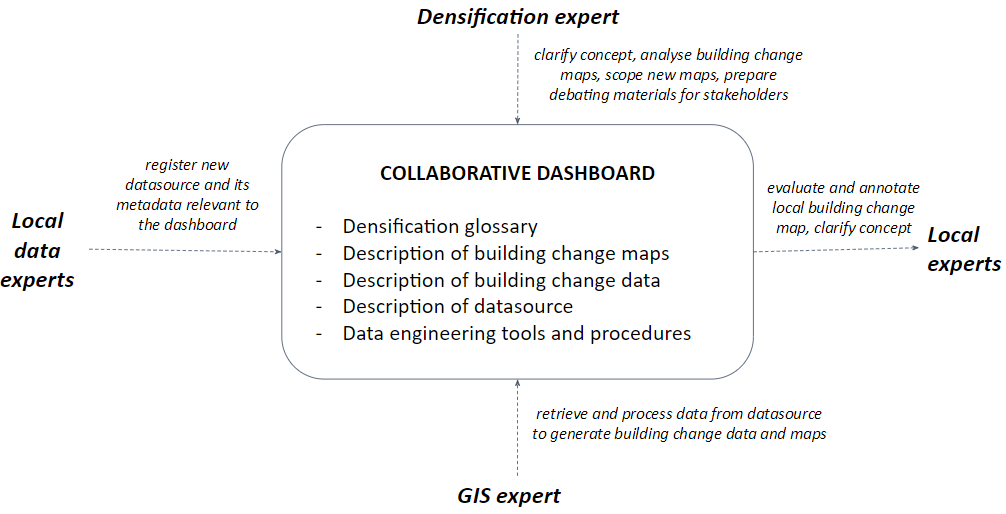
\includegraphics[width=\linewidth]{figures/dashboard_concept.png}\smallskip

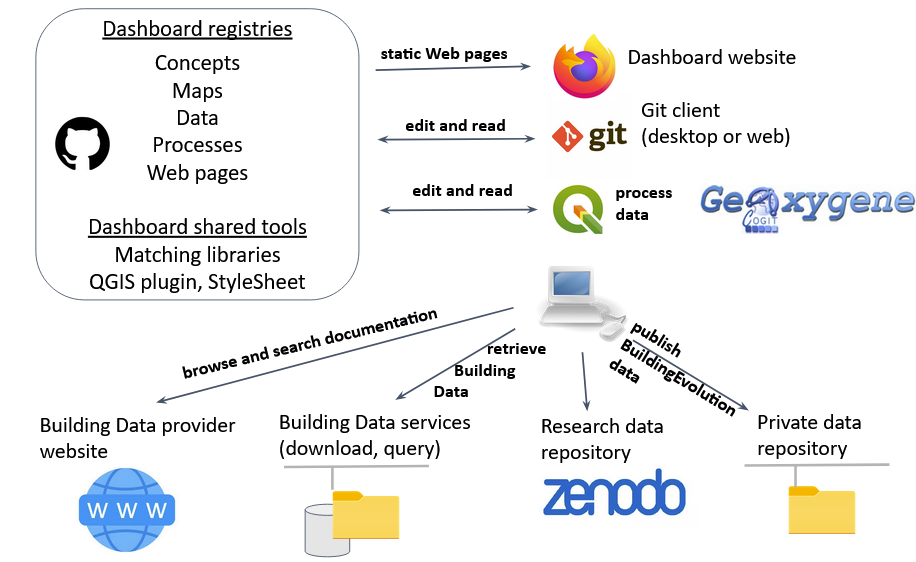
\includegraphics[width=\linewidth]{figures/dashboard.png}

\end{column}
\begin{column}{0.4\linewidth}
	
	\footnotesize	
	
	\justify	
	
	Preliminary work aimed at harmonising operationnal concepts and data sources qualification across the different countries:
	
	\bigskip
	
	$\rightarrow$ git-based dashboard to share knowledge and resources between different types of experts	\cite{bucher2024conceptualising}
	
	\bigskip
	
	$\rightarrow$ reproducible tools and methods, including \textbf{building change detection scripts} 	
	
\end{column}

\end{columns}

}


\sframe{Difficulties with data for building change}{




\begin{center}
	
	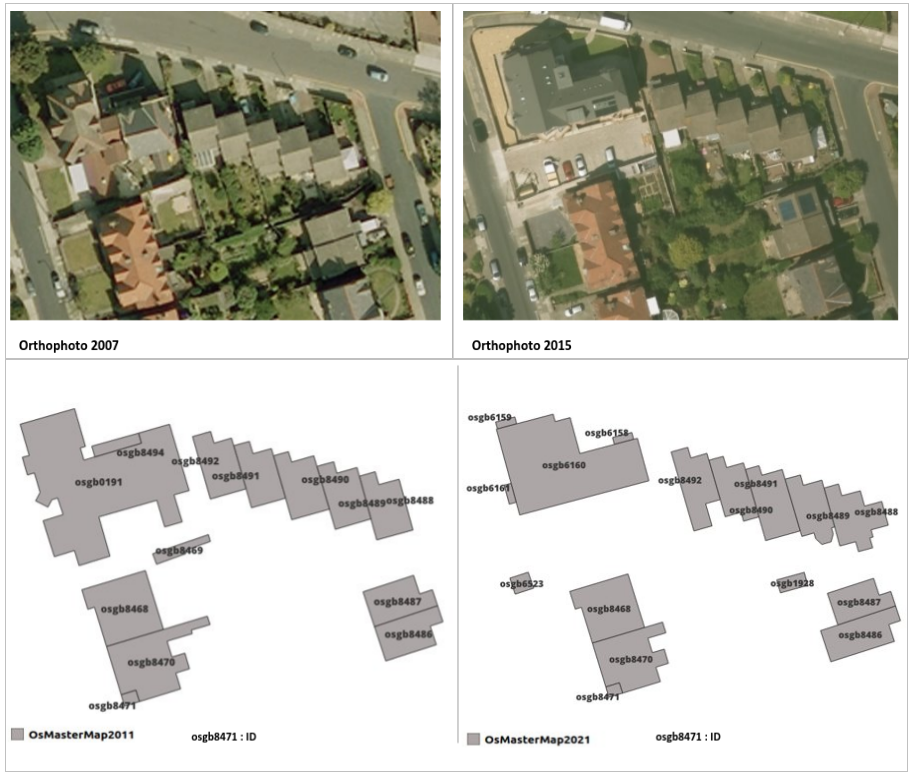
\includegraphics[width=0.75\linewidth]{figures/buildingchange_1.png}	
	
\end{center}

\footnotesize

\textit{Example in the UK where changes in OSMasterMap building data includes both real changes and data changes.} Source: \cite{bucher2025building}

}


\sframe{Difficulties with data for building change}{

\begin{center}
	
	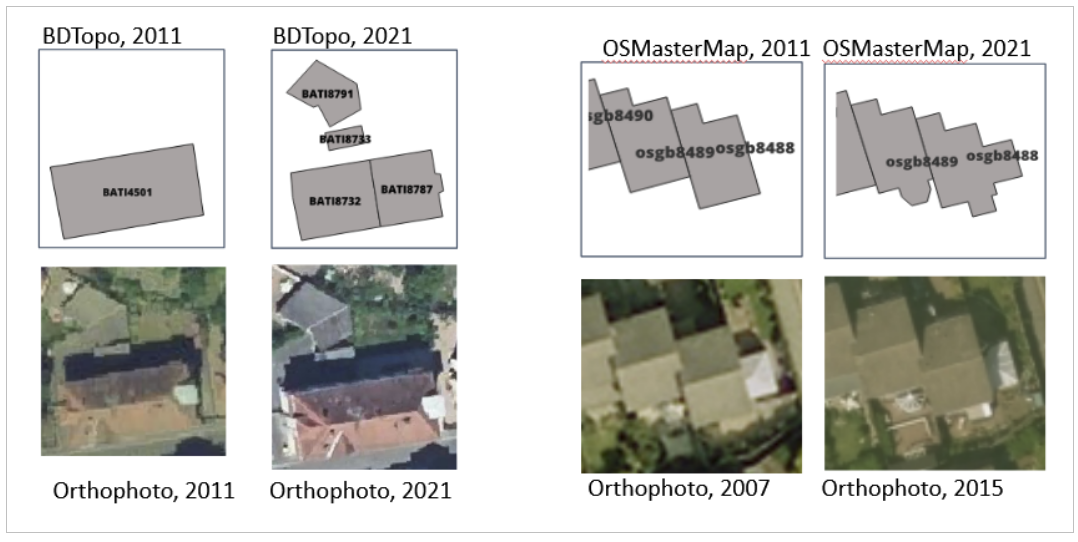
\includegraphics[width=\linewidth]{figures/buildingchange_2.png}	
	
\end{center}

\footnotesize

\textit{Example of data specification changes only, for France (BDTopo) and the UK (OSMasterMap).} Source: \cite{bucher2025building}

}


\begin{frame}{Quantifying building change}

% Raster data such as aerial imagery, on which machine learning methods provide a good performance for land-use change for example \cite{khelifi2020deep}, is not sufficient for that purpose, and change detection must be performed on vector data of building geometries. To that purpose, geospatial vector data matching algorithms are an efficient tool \cite{xavier2016survey}, with the advantage of being robust to spatial noise in geometries and changes in data specifications. They however require some extensive parametrisation and provide varying performances \cite{guardiola2024optimising}.

%\justify

$\rightarrow$ Machine Learning on remote sensing raster data had improved performance in recent years, but remains not robust enough in terms of quality and resolution for that particular purpose \cite{khelifi2020deep}

\medskip

$\rightarrow$ Geospatial vector data matching algorithms as a method for change detection \cite{xavier2016survey}, applied to linear data \cite{costes2015aggregated} and polygonal data \cite{gregory2007historical}.

\medskip

$\rightarrow$ A new algorithm combining Geometric Matching of Areas \cite{belhadjali:tel-03244834} with Multi-criteria Matching \cite{olteanu2015knowledge} presented at CCS last year \cite{guardiola2024optimising}.

\end{frame}


\sframe{Research objective}{



%An important issue for optimising this type of algorithms is the lack of ground-truth datasets with a large enough size and diversity. We propose in this contribution to tackle this issue, for the specific case of building change detection.

%We therefore introduce a web application designed to annotate potential matching links between two vector datasets.



$\rightarrow$ Vector Matching algorithm require extensive parametrisation and optimisation, and provide varying performances in different context.

\medskip

$\rightarrow$ Need for large and specific ground-truth datasets (building layers annotated with expected links).

\bigskip

\textbf{Research objective:}

\textit{Design and develop a web application designed to annotate potential matching links between two vector dataset.}


}



\begin{frame}{Functionalities of the annotation web-application}

% Its main functionalities are that (i) it is fully based on git and javascript, requiring no database nor advanced web server deployment, and can be automatically deployed through github pages for example; (ii) it manages multi-user collaboration, with authentication linked to rights granted for the project git repository (implemented only for github for now); (iii) provides a dashboard with the user progress and the overall progress on all datasets displayed on maps; (iv) it allows collaborators annotating two vector datasets at two different dates, with aerial photographs being provided in the background for ground-truthing.

\footnotesize

\begin{itemize}
	\item fully based on git and javascript: no database nor server management, automatically deployed through github pages
	\item handles multi-user collaboration, with authentication given by writing rights on the git repository
	\item provides a dashboard to summarise user progress and overall progress
	\item allows annotation of two vector datasets, with aerial photographs being provided in the background for ground-truthing
\end{itemize}

\smallskip


\begin{center}
  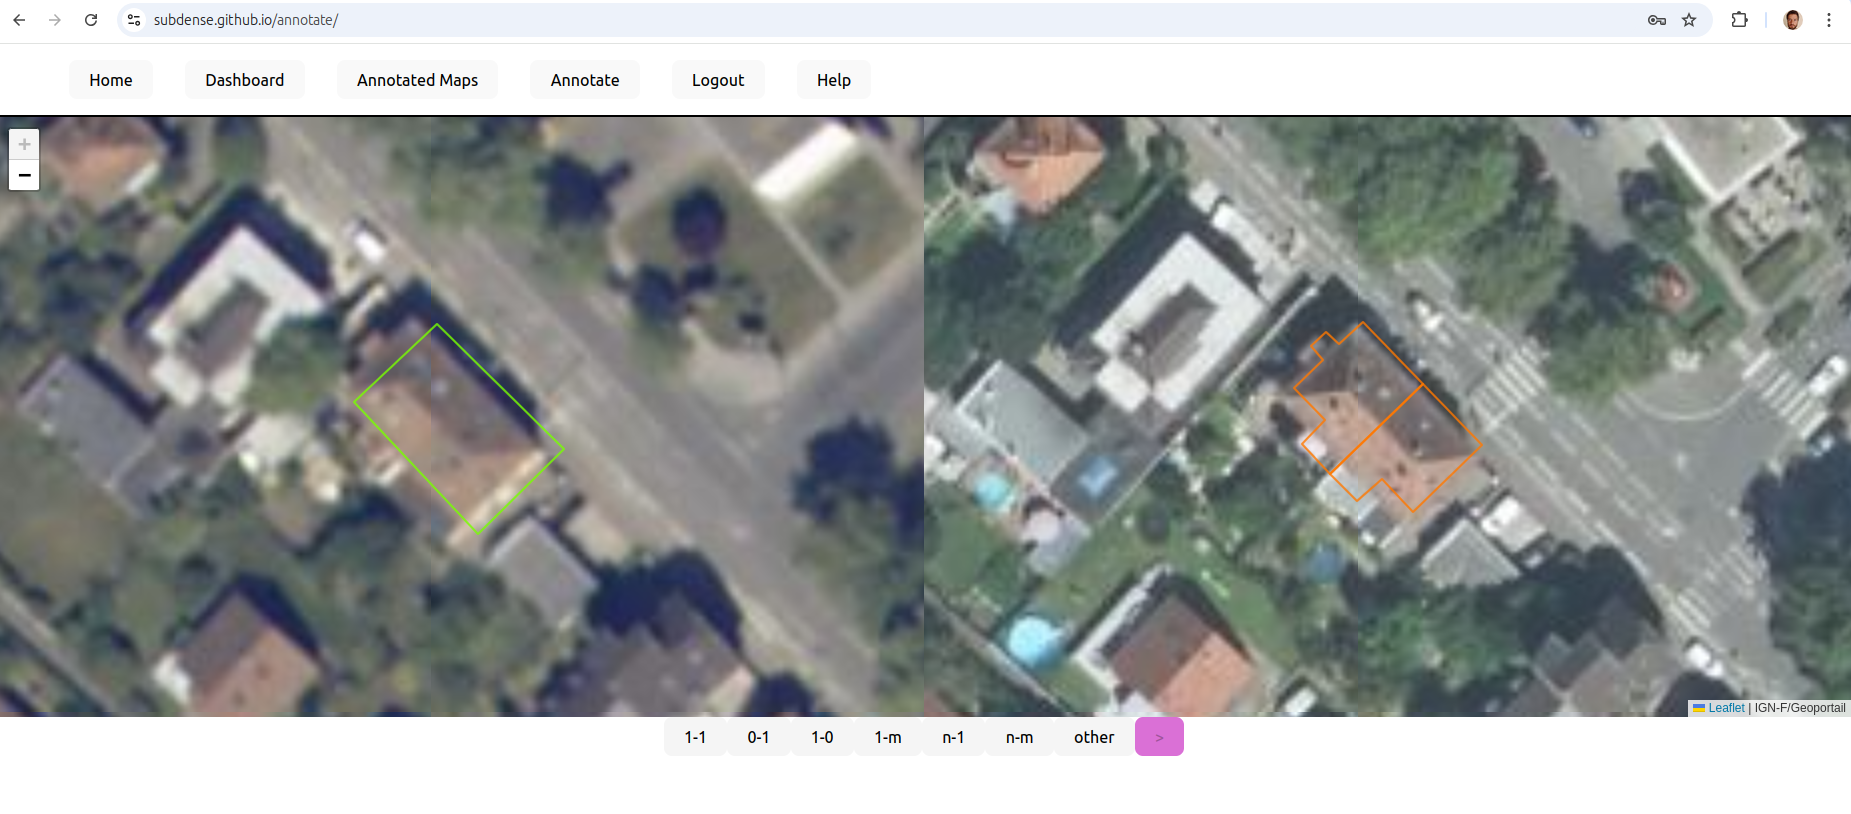
\includegraphics[width=\linewidth]{figures/annotator.png}
\end{center}



\end{frame}


\begin{frame}{Two stage annotation process}

%The annotation is sequential on potential matching links (intersecting features between the two datasets), and the user must ground-truth first the type of link the algorithm should detect (no link, single, multiple), then the type of real world evolution (parametrised for building changes in our case), and can also highlight and comment data quality issues. 

%  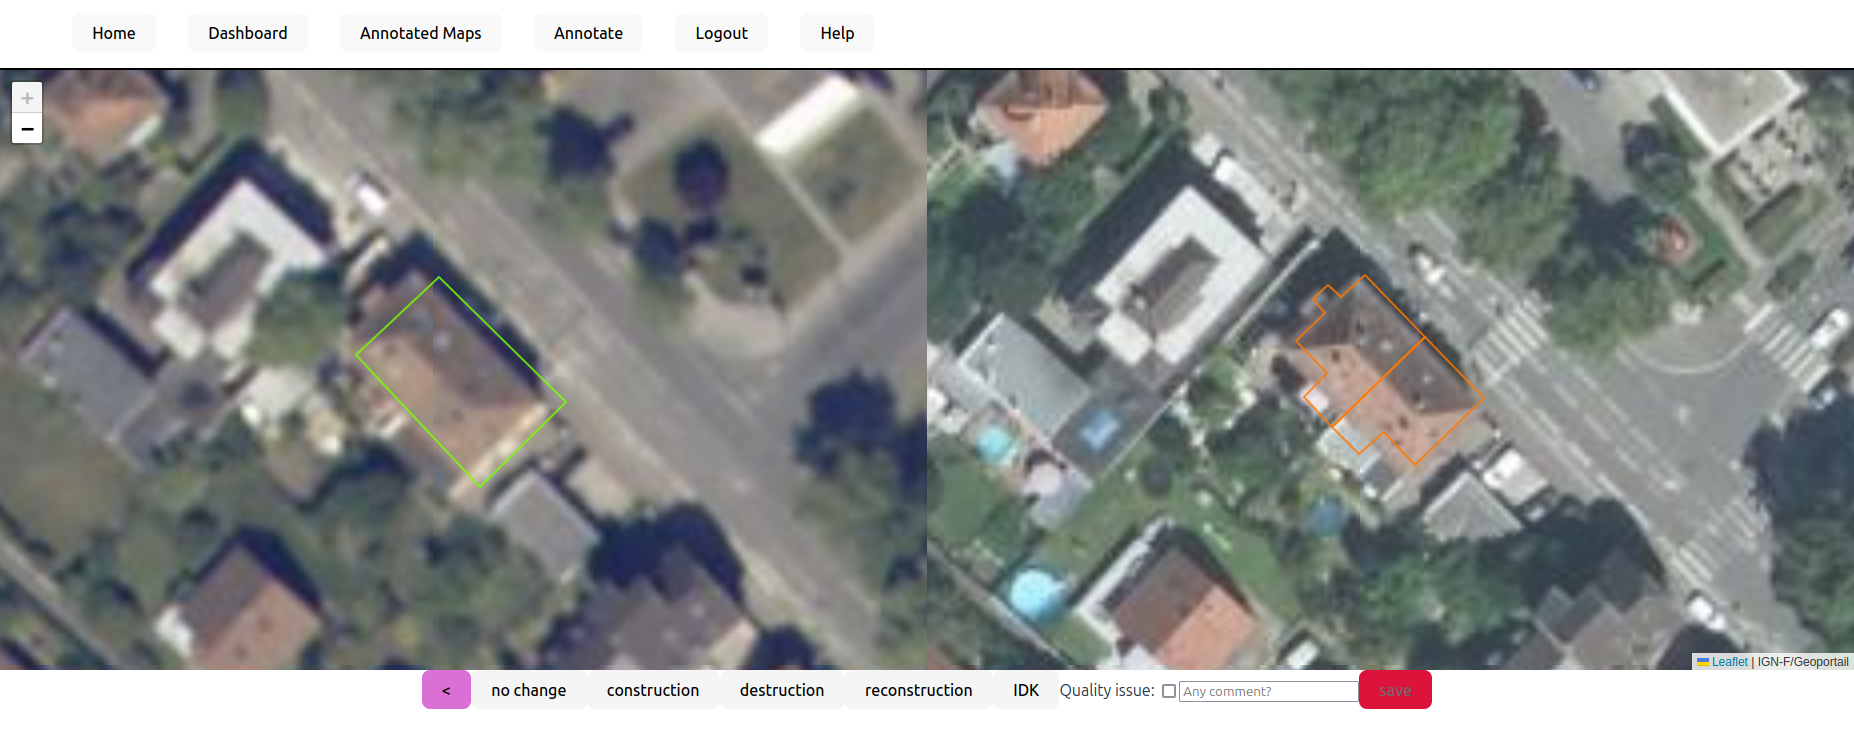
\includegraphics[width=\textwidth]{figures/example_annotate_2025-03-20_22-27-20.png}
%  \caption{Screenshot of the annotation web application. On the top the user can access the different tabs, such as the dashboard with the annotation progress on the tasks ths user was assigned, or global maps showing progress across all users and datasets in space. The main tab to annotate shows two aerial photographs of the same place at the two compared dates, with the vector features at each date surimposed. In this particular case, there seems to be no change in the real world, but the polygon data for buildings significantly changed. The user first provides the type of link, and then (shown in the screenshot) the type of real world building change (no change, construction, destruction, reconstruction, does not know), and can comment on a data quality issue. Note that aerial photographs are in some rare cases not enough to ground-truth change, thus the option to skip the step. Once clicking ``save'', the next unit to annotate will be displayed.}

\footnotesize

\begin{center}
  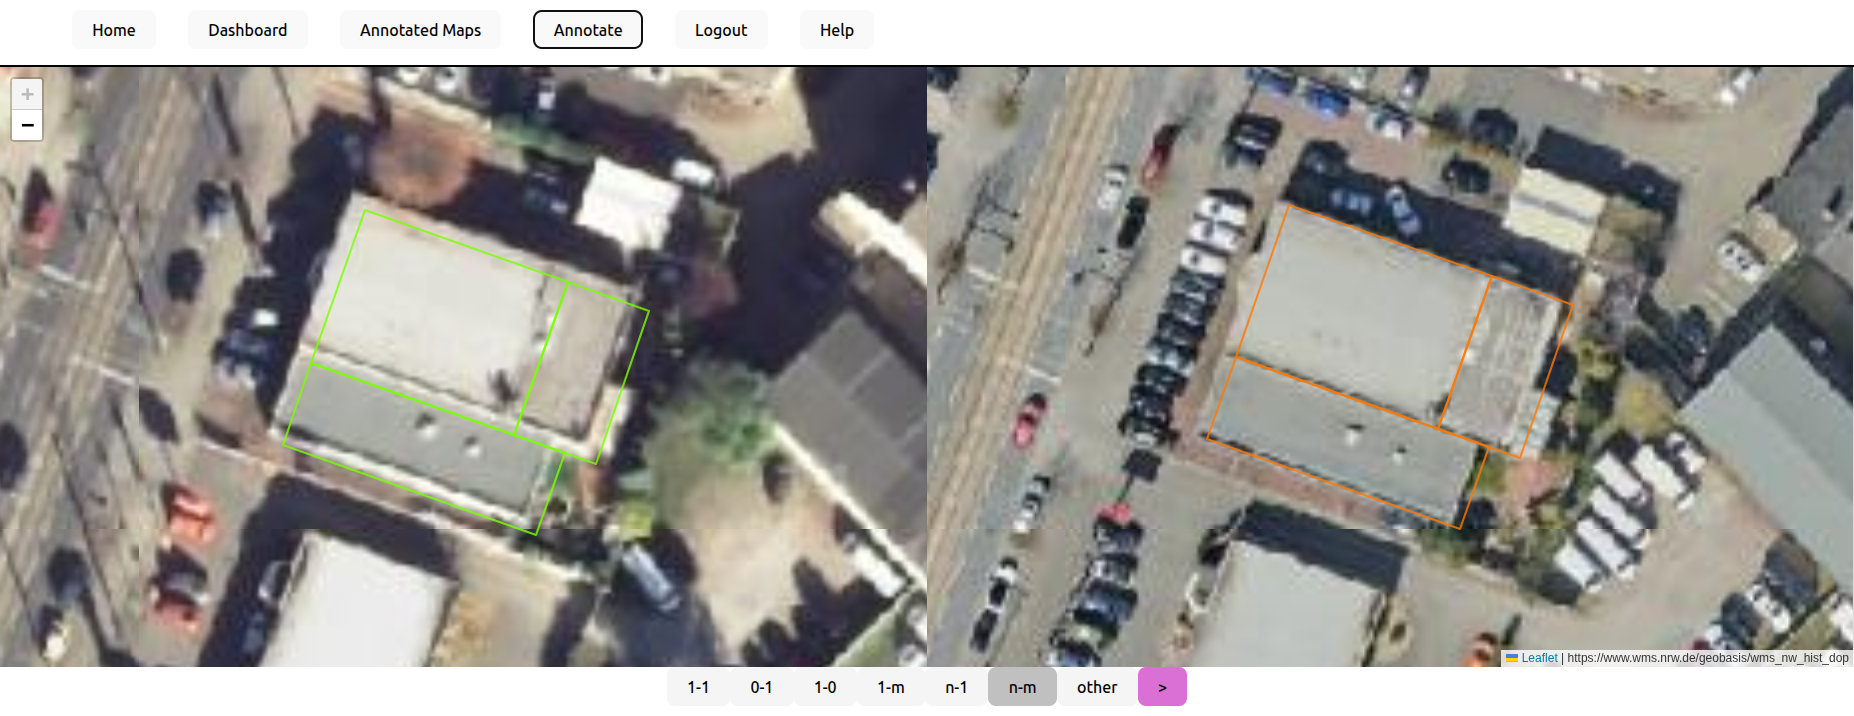
\includegraphics[width=0.65\linewidth]{figures/example_dortmund_nochange_stage1.png}
\end{center}

\textbf{Stage 1:} type of matching link (1-1, 0-1, 1-0, 1-m, n-1, n-m).

\smallskip

\begin{center}
  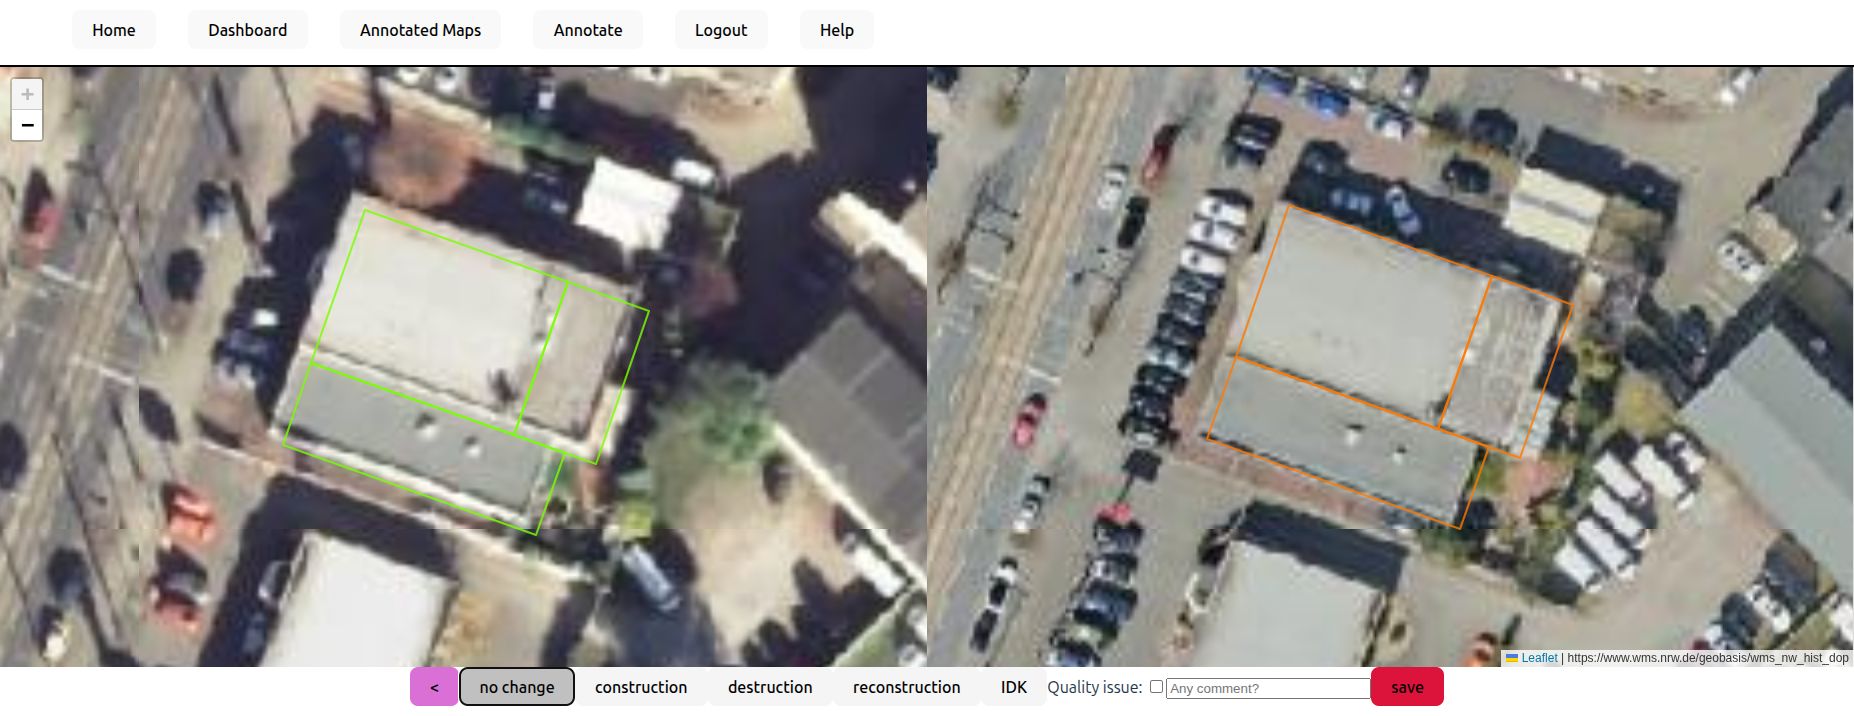
\includegraphics[width=0.65\linewidth]{figures/example_dortmund_nochange_stage2.png}
\end{center}

\textbf{Stage 1:} type of real word evolution (no change, construction, destruction, reconstruction, don't know), signal a quality issue and comment.



\end{frame}



\begin{frame}{Dashboard and maps to monitor progress}

\begin{center}
	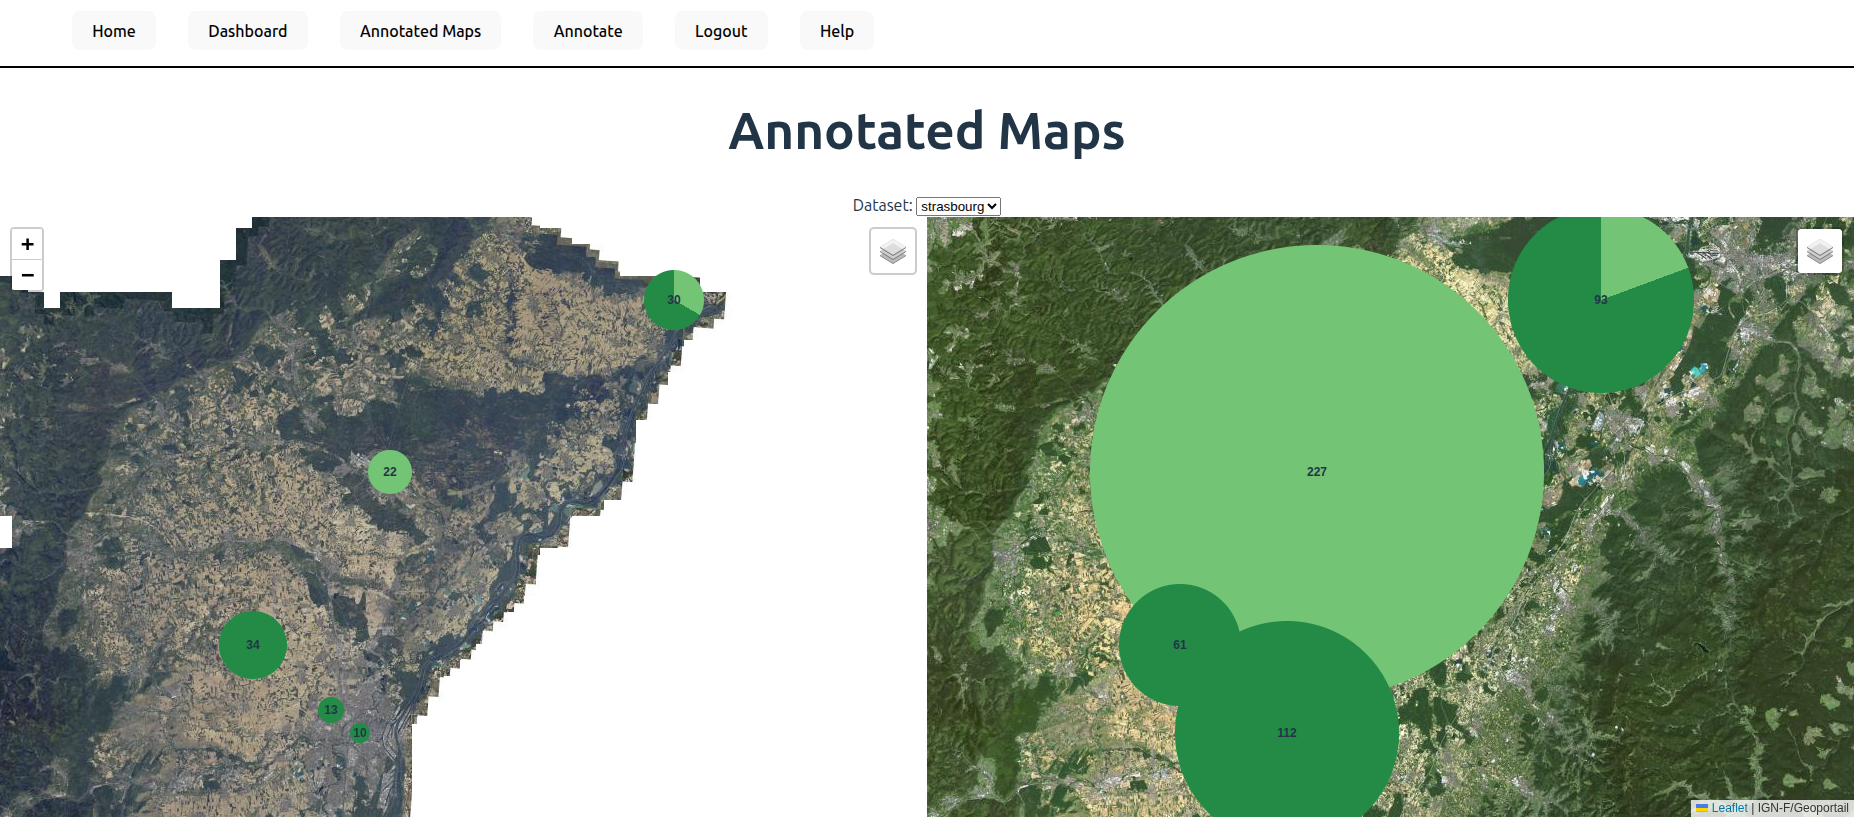
\includegraphics[width=\linewidth]{figures/example_annotatordashboard.png}
\end{center}

\end{frame}



\begin{frame}{Architecture}

%The application is open source and available at \url{https://github.com/subdense/annotate}.
%We show an example of the application in Figure 1


% git-based archi


\end{frame}



\begin{frame}{Deployment}

%We currently deployed the application on samples within the functional urban areas of Strasbourg, France and Dortmund, Germany, as data quality issues are very different across countries (for example, French BDTopo had a specification change in 2015 leading to many geometry changes with polygon splits that do not correspond to real-world changes). We compare buildings between 2011 and 2021, for all buildings within 500m radius circles around 100 sampled points for each area. The annotation campaign is currently ongoing with several researchers experts on GIS data and urban densification.




% example and/or demo

\end{frame}


\begin{frame}{Work in progress: algorithm optimisation}

%First results to optimise algorithms (in the sense of F-score for real-world change prediction) with partial ground-truth datasets were obtained for the same algorithms studied by \cite{guardiola2024optimising} (the Multi-criteria matching algorithm and the Geometric Matching of Areas algorithm), and confirm previous results obtained with synthetic data, in particular that (i) each algorithm can be optimised to better perform in different urban form typologies (center, housing projects, suburbs); (ii) they can be combined into a multi-modelling approach for a better overall performance.

%Our contribution thus provide a basis for a robust quantification of urban densification at the building level, and a generic web application to annotate vector datasets in a comparative way.

% WIP optim with OpenMOLE
% $\rightarrow$ work in progress: large annotation campaign for the 6 case study cities in the 3 countries


\end{frame}





\sframe{Perspectives}{

% pymatch lib
% ground truth datasets to be published
% optimise combined algo - benchmark systematically with others

\footnotesize
%
%\textbf{Contributions: }
%\begin{itemize}
%	\item a benchmark of algorithms \cite{guardiola2024benchmarking}
%	\item a new algorithm combining GMoA and MCA \cite{guardiola2024optimising}
%	\item open source python library \url{https://github.com/umrlastig/pymatch}
%	\item web app to annotate links \url{https://github.com/subdense/annotate}
%\end{itemize}

%\textbf{Work in progress: } % aka necessary for solid paper

%\begin{itemize}
%	\item annotation campaign to produce a large scale ground-truth dataset
%	\item optimisation using the ground truth in OpenMOLE
%	\item systematic exploration and validation using the synthetic data generator
%	\item include other matching algorithms in the benchmark % at least one well established in the literature
%\end{itemize}

%\textbf{Perspectives: }

%\begin{itemize}
%	\item extension to line and points matching algorithms
%	\item use for data quality issues
%\end{itemize}


%The application is currently parametrised for building change, but vector data sources, aerial imagery sources, and change labels can all be customised in a configuration file, and thus can be changed for other types of features, such as land plots or road networks


%\url{https://github.com/subdense/annotate}



}







%%%%%%%%%%%%%%%%%%%%%
\begin{frame}[allowframebreaks]
\frametitle{References}
\bibliographystyle{apalike}
\bibliography{biblio}
\end{frame}
%%%%%%%%%%%%%%%%%%%%%%%%%%%%



\begin{frame}{Reserve slides}

\vfill

\begin{center}
{\Huge\bf Reserve slides}
\end{center}

\vfill

\end{frame}



\begin{frame}{The SUBDENSE project}


\begin{columns}
	\begin{column}{0.6\textwidth}
		The SubDense European project studies the dynamics of suburban densification by:
 
	\end{column}
	\begin{column}{0.4\textwidth}
		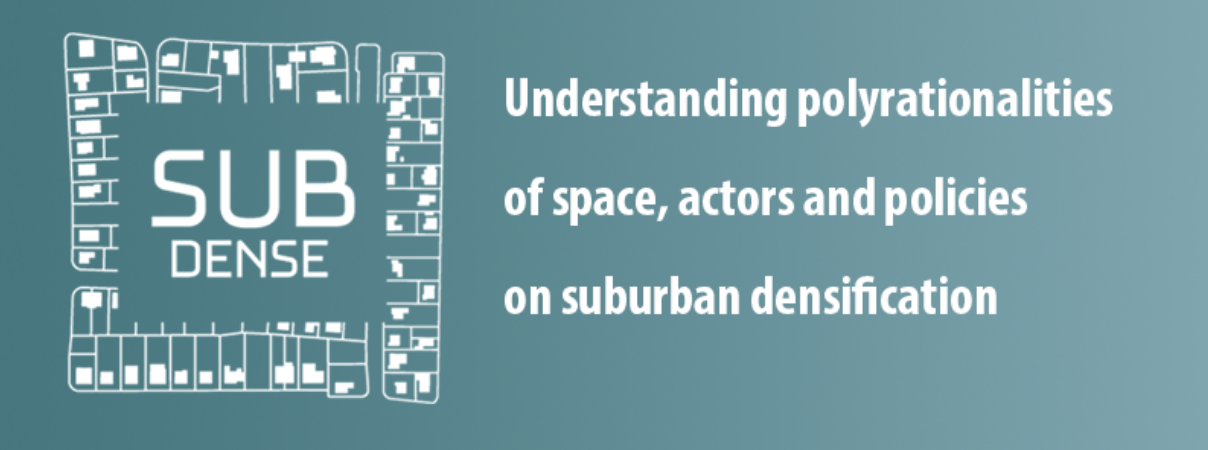
\includegraphics[height=0.2\textheight]{figures/subdense.png}
	\end{column}
\end{columns}


\begin{itemize} 
	\item exploring how diverse strategies of land policy interact with landowners’ and local stakeholders’ interest and agency to shape suburban densification and their impact on suburbia across different planning systems (France, Germany, UK);
	\item combining quantitative approaches (geodata analysis and geosimulation) with qualitative approaches (social and policy science and planning).
\end{itemize}



\includegraphics[height=0.1\textheight]{figures/logos.png}\hspace{-0.1cm}

\includegraphics[height=0.1\textheight]{figures/tud.png}



\end{frame}



\sframe{Geometric Matching of Areas (GMoA) algorithm}{

\begin{columns}
  \begin{column}{0.4\textwidth}
  		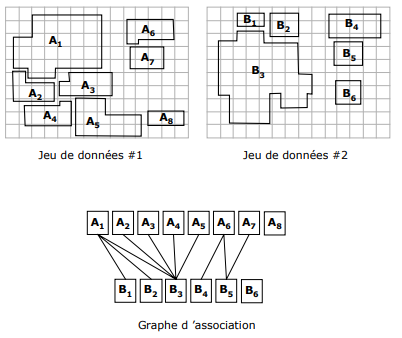
\includegraphics[width=\linewidth]{figures/GMoA_1.png}
	\smallskip
	  	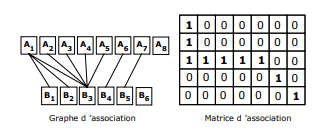
\includegraphics[width=\linewidth]{figures/GMoA_2.png}	
  		
  \end{column}
   \begin{column}{0.6\textwidth}
   
	\footnotesize   
   
  	 Algorithm to produce m-n links based only on geometries \cite{harvey1998geometric} \cite{belhadjali:tel-03244834}:
  	 
	\begin{enumerate}
		\item Construct all possible association links as surfaces with a non-empty intersection (top left Fig.)
		\item Filter links with an intersection surface below a threshold parameter
		\item Filter links with an intersection surface too small relatively to matched surfaces (rate parameter)
		\item Construct all m-n links as connected clusters in the remaining bipartite graph (bottom left Fig.)
	\end{enumerate}	  	 
  	 
  \end{column}
\end{columns}

\bigskip

\footnotesize

$\rightarrow$ implemented in the \texttt{geoxygene} java library \cite{bucher2012geoxygene} by \cite{mustiere2002description}



}

\sframe{Application of the GMoA to change detection}{

% -> code python shared through the dashboard

\begin{center}
  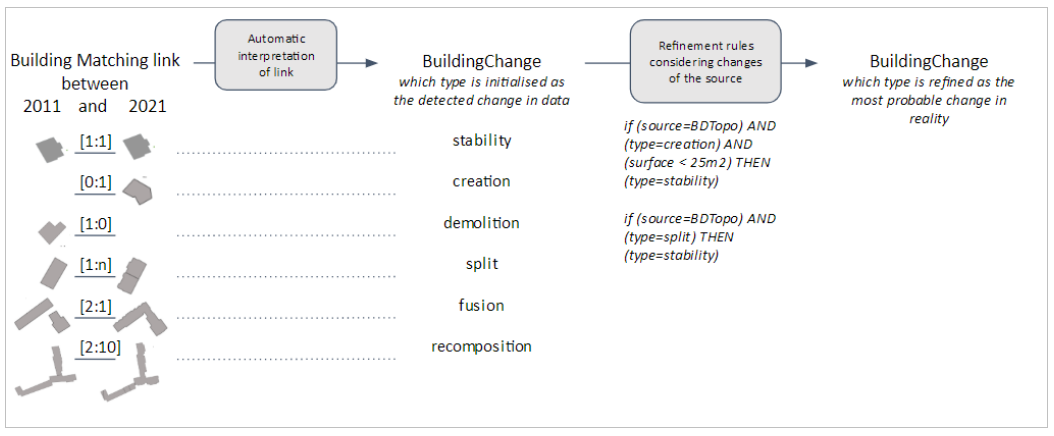
\includegraphics[width=\linewidth]{figures/change.png}
\end{center}

\bigskip

Automatic interpretation of matching links into building change, with specific adjustements for BDTopo \cite{bucher2025building}, by a \texttt{python} script available at \url{https://github.com/subdense/matching}


}


\sframe{Example}{

% Strasbourg?


\begin{center}
  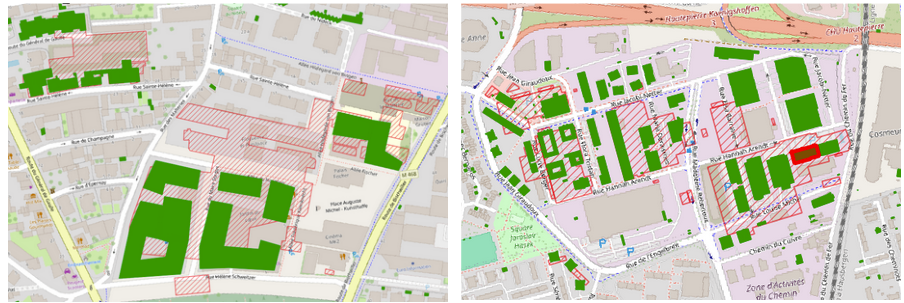
\includegraphics[width=\linewidth]{figures/buildingchange_gmoa.png}
\end{center}

\bigskip

Building evolution for two examples in the urban area of Strasbourg \cite{bucher2025building} 

}


\sframe{Multi-criteria matching algorithm (MCA)}{



\begin{center}
  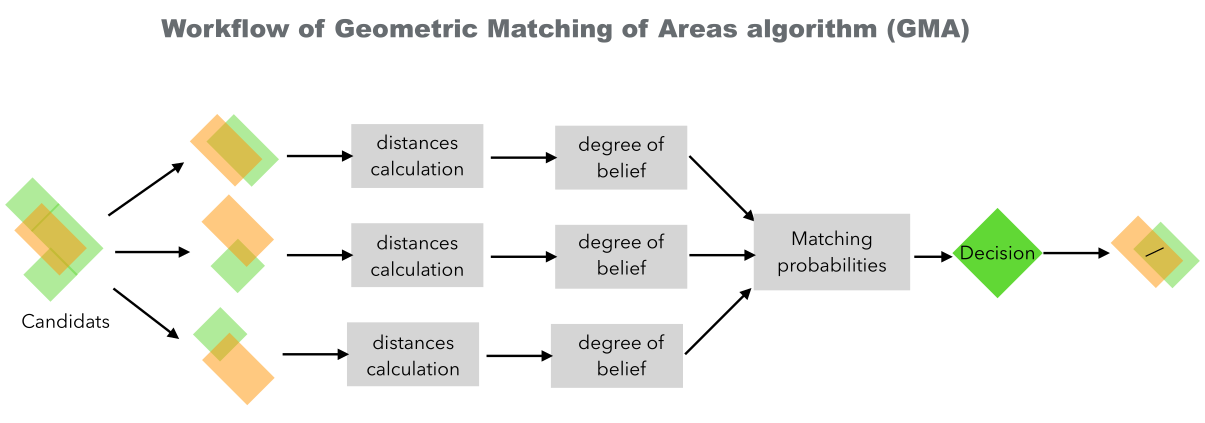
\includegraphics[width=\linewidth]{figures/mca.png}
\end{center}

\bigskip

Implementation of the Multi-criteria matching algorithm \cite{olteanu2015knowledge} in python by \cite{guardiola2024benchmarking}, with euclidian, surface, radial and Hausdorff distances, and run twice to obtain m-n links.

}


\sframe{Benchmarking of algorithms}{

% paper frccs 2024 -> optimal params for a compromise perf/time

\begin{center}
  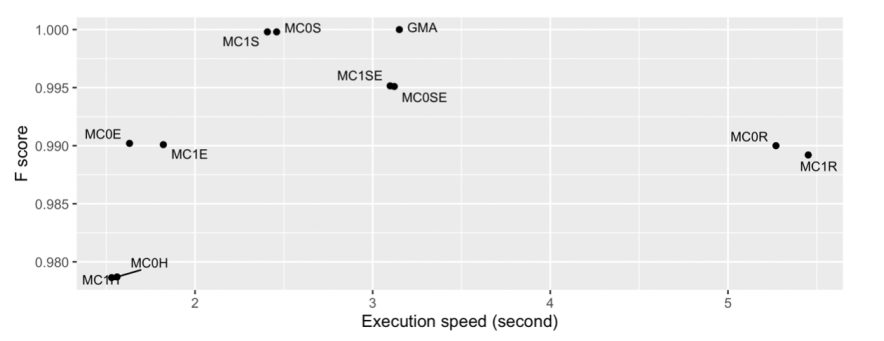
\includegraphics[width=\linewidth]{figures/benchmark.png}
\end{center}

\bigskip

\footnotesize

Bi-objective benchmark optimising for performance (F-score on a $\simeq$ 2k buildings ground truth dataset) and runtime, for different parametrisations of the two algorithms, by \cite{guardiola2024benchmarking}

$\rightarrow$ various algorithm performances

% We find an under-detection for the GMA and an over-detection for MCA
% GMA is a well method for n-m links rather than MCA is better for 1-1 links

$\rightarrow$ under-detection of change by GMoA and over-detection by MCA

$\rightarrow$ GMA better for m-n links, MCA better for 1-1 links


}


\sframe{A new algorithm using multi-modeling}{

% cite CCS2024

\begin{center}
  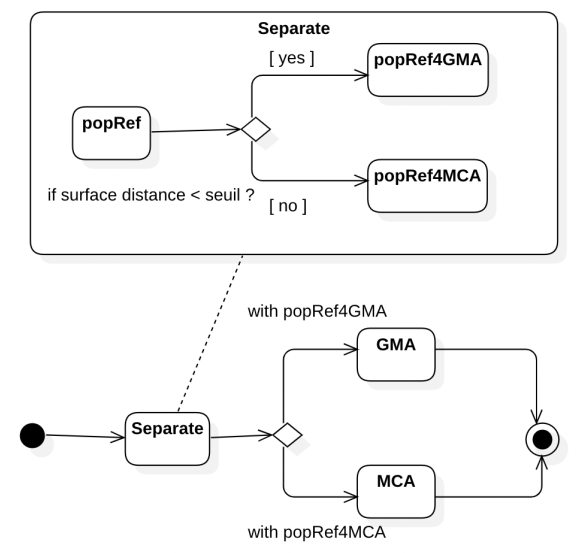
\includegraphics[width=0.6\linewidth]{figures/algo.png}
\end{center}

\bigskip

\footnotesize


Proposition of a new algorithm combining GMoA and MCA, with the choice made through thresholding surface distance \cite{guardiola2024optimising}

}


\sframe{Example}{

% Rennes


\begin{center}
  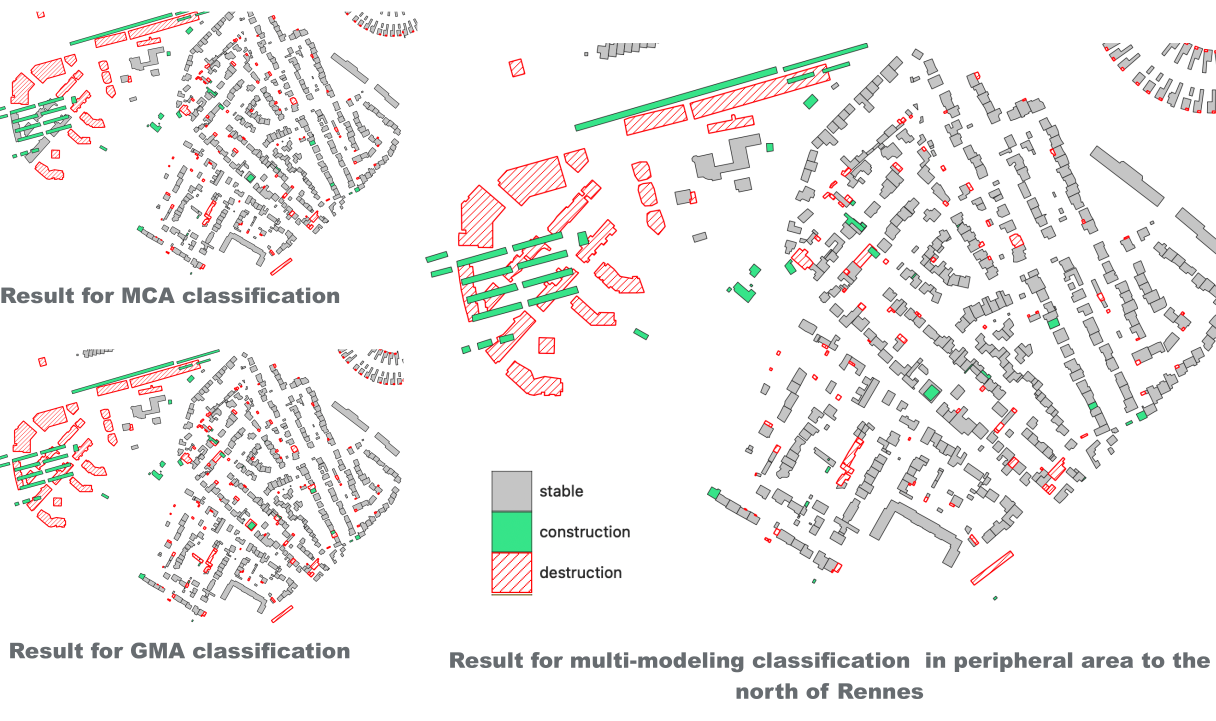
\includegraphics[width=\linewidth]{figures/result_algo.png}
\end{center}

\bigskip

%\footnotesize


Results obtained on an example in the suburbs of Rennes \cite{guardiola2024optimising}

}



\sframe{Validating the algorithm with synthetic data}{

% and optimising


\begin{center}
  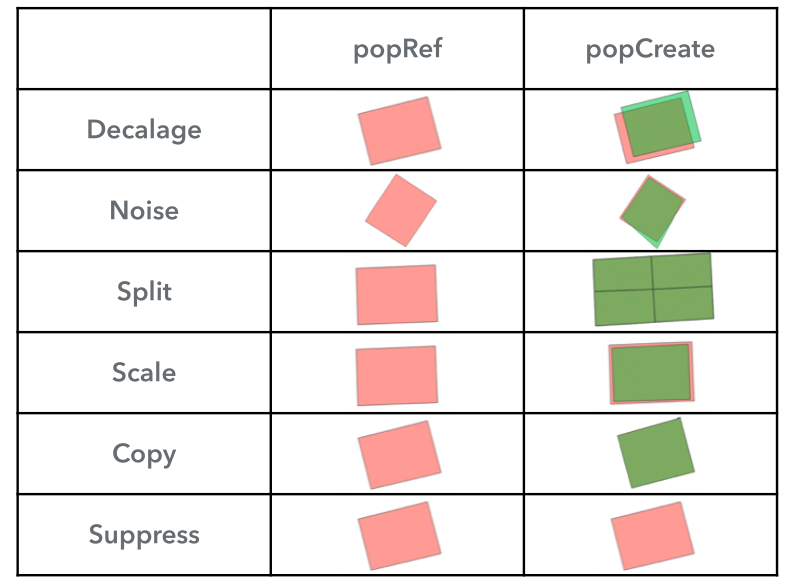
\includegraphics[width=0.63\linewidth]{figures/synthdata_1.png}
  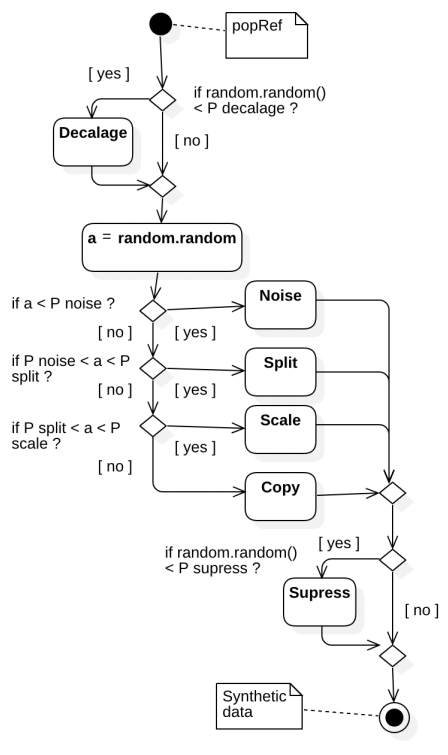
\includegraphics[width=0.27\linewidth]{figures/synthdata_2.png}
\end{center}

\bigskip

\footnotesize

Synthetic data generator introduced by \cite{guardiola2024optimising} to generate datasets on which to validate and optimise the algorithm

}


\sframe{First results on synthetic data}{

% integrated into OpenMOLE


\begin{center}
  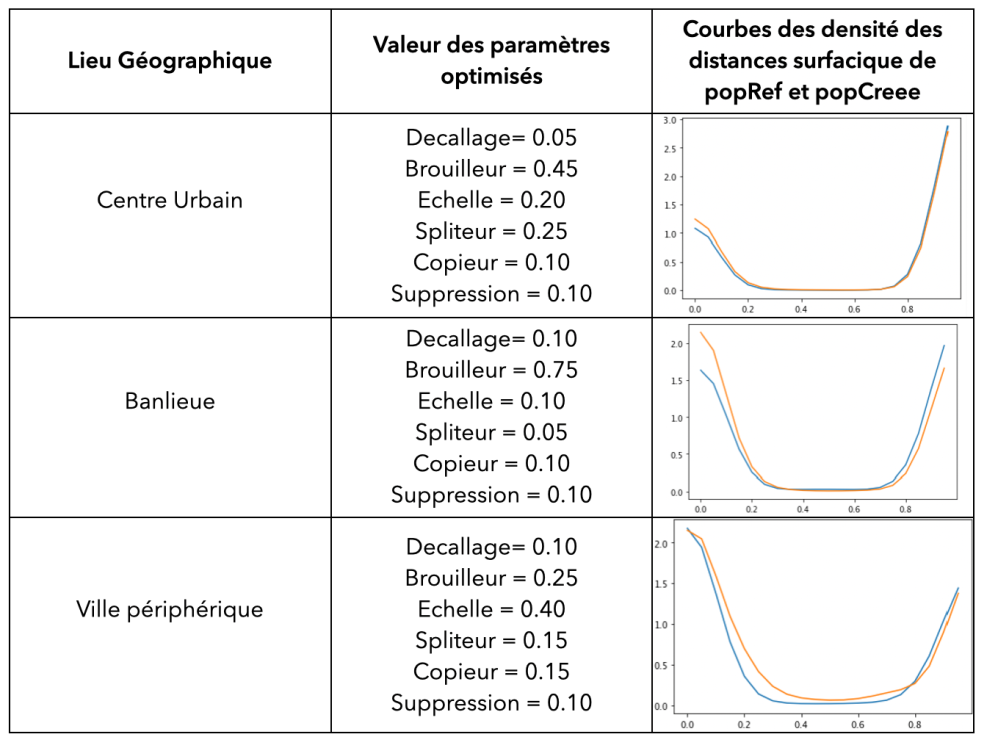
\includegraphics[width=0.75\linewidth]{figures/synthdata_calib.png}
\end{center}

\bigskip

\footnotesize

Integration into the OpenMOLE software and calibration of the generator for different urban typologies (single fitness: distance between surface distance densities) \cite{guardiola2024optimising}

}








\end{document}

